\documentclass[a4paper]{article}  

\usepackage{mathtools}
\usepackage{amsthm}
\usepackage{amssymb}
\usepackage{tikz}
\usepackage{algpseudocode}

\title{CS270 Homework 4}
\author{Valkyrie Savage \thanks{Shiry, Mitar, Orianna, Peggy, Jan Vondr\'{a}k of Stanford, stat.ethz.ch, Wikipedia}}

\begin{document}
\maketitle

\begin{enumerate}

\item Maximum weight bipartite matching
	\begin{enumerate}
		\item For example:\\
		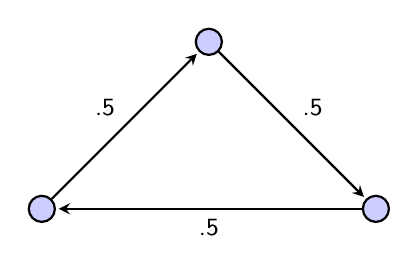
\begin{tikzpicture}[->,>=stealth,shorten >=1pt,auto,node distance=3cm,
 		thick,main node/.style={circle,fill=blue!20,draw,font=\sffamily\Large\bfseries}]

  		\node[main node] (B) {};
  		\node[main node] (A) [below left of=B] {};
  		\node[main node] (C) [below right of=B] {};

  		\path[every node/.style={font=\sffamily\small}]
    		(A) edge node {.5} (B)
        		(B) edge node {.5} (C)
        		(C) edge node {.5} (A);
		\end{tikzpicture}
		\item 
			\begin{align}
				\max \sum_e{w_e x_e}\\
				\forall v \in V : \sum_{e=(u,v)} {x_e} &\leq 1 \\
				x_e &\geq 0 \\
				 \forall U \subseteq V s.t. \left|{U}\right| = 2k+1 , k \in \{0,1,2,...\} :
					\sum_{E(U)}{x_e} &= k
			\end{align}

		\item The dual of the linear program:
			\begin{align}
				\min \sum
			\end{align}
	\end{enumerate}

\item Convex bodies
	\begin{enumerate}
		\item We have two bodies, $A$ and $B$.  We select a point $a \in A$ where $a$ is the closest point in $A$ to $B$ and a point $b \in B$ where $b$ is the closest point in $B$ to $A$.  We construct a hyperplane between $a$ and $b$.  If the hyperplane intersects $A$ at a point $a_1$, then we know that $a$ was not, in fact, the closest point in $A$ to $B$.  Similarly, if the hyperplane intersects $B$ at a point $b_1$, then we know that $b$ was not, in fact, the closest point in $B$ to $A$.
		\item Farkas B states that there is a solution for exactly one of
			\begin{enumerate}
				\item $Ax \leq b$
				\item $y^TA=0, y^Tb<0, y \geq 0$
			\end{enumerate}
			So look at the geometric interpretations.  Either we are inside the body or there is a separating hyperplane y.
	\end{enumerate}

\item Facility Location

\item Relational database joins

\item Project description
\end{enumerate}
\end{document}